% Options for packages loaded elsewhere
\PassOptionsToPackage{unicode}{hyperref}
\PassOptionsToPackage{hyphens}{url}
%
\documentclass[
]{article}
\usepackage{amsmath,amssymb}
\usepackage{iftex}
\ifPDFTeX
  \usepackage[T1]{fontenc}
  \usepackage[utf8]{inputenc}
  \usepackage{textcomp} % provide euro and other symbols
\else % if luatex or xetex
  \usepackage{unicode-math} % this also loads fontspec
  \defaultfontfeatures{Scale=MatchLowercase}
  \defaultfontfeatures[\rmfamily]{Ligatures=TeX,Scale=1}
\fi
\usepackage{lmodern}
\ifPDFTeX\else
  % xetex/luatex font selection
\fi
% Use upquote if available, for straight quotes in verbatim environments
\IfFileExists{upquote.sty}{\usepackage{upquote}}{}
\IfFileExists{microtype.sty}{% use microtype if available
  \usepackage[]{microtype}
  \UseMicrotypeSet[protrusion]{basicmath} % disable protrusion for tt fonts
}{}
\makeatletter
\@ifundefined{KOMAClassName}{% if non-KOMA class
  \IfFileExists{parskip.sty}{%
    \usepackage{parskip}
  }{% else
    \setlength{\parindent}{0pt}
    \setlength{\parskip}{6pt plus 2pt minus 1pt}}
}{% if KOMA class
  \KOMAoptions{parskip=half}}
\makeatother
\usepackage{xcolor}
\usepackage[margin=1in]{geometry}
\usepackage{color}
\usepackage{fancyvrb}
\newcommand{\VerbBar}{|}
\newcommand{\VERB}{\Verb[commandchars=\\\{\}]}
\DefineVerbatimEnvironment{Highlighting}{Verbatim}{commandchars=\\\{\}}
% Add ',fontsize=\small' for more characters per line
\usepackage{framed}
\definecolor{shadecolor}{RGB}{248,248,248}
\newenvironment{Shaded}{\begin{snugshade}}{\end{snugshade}}
\newcommand{\AlertTok}[1]{\textcolor[rgb]{0.94,0.16,0.16}{#1}}
\newcommand{\AnnotationTok}[1]{\textcolor[rgb]{0.56,0.35,0.01}{\textbf{\textit{#1}}}}
\newcommand{\AttributeTok}[1]{\textcolor[rgb]{0.13,0.29,0.53}{#1}}
\newcommand{\BaseNTok}[1]{\textcolor[rgb]{0.00,0.00,0.81}{#1}}
\newcommand{\BuiltInTok}[1]{#1}
\newcommand{\CharTok}[1]{\textcolor[rgb]{0.31,0.60,0.02}{#1}}
\newcommand{\CommentTok}[1]{\textcolor[rgb]{0.56,0.35,0.01}{\textit{#1}}}
\newcommand{\CommentVarTok}[1]{\textcolor[rgb]{0.56,0.35,0.01}{\textbf{\textit{#1}}}}
\newcommand{\ConstantTok}[1]{\textcolor[rgb]{0.56,0.35,0.01}{#1}}
\newcommand{\ControlFlowTok}[1]{\textcolor[rgb]{0.13,0.29,0.53}{\textbf{#1}}}
\newcommand{\DataTypeTok}[1]{\textcolor[rgb]{0.13,0.29,0.53}{#1}}
\newcommand{\DecValTok}[1]{\textcolor[rgb]{0.00,0.00,0.81}{#1}}
\newcommand{\DocumentationTok}[1]{\textcolor[rgb]{0.56,0.35,0.01}{\textbf{\textit{#1}}}}
\newcommand{\ErrorTok}[1]{\textcolor[rgb]{0.64,0.00,0.00}{\textbf{#1}}}
\newcommand{\ExtensionTok}[1]{#1}
\newcommand{\FloatTok}[1]{\textcolor[rgb]{0.00,0.00,0.81}{#1}}
\newcommand{\FunctionTok}[1]{\textcolor[rgb]{0.13,0.29,0.53}{\textbf{#1}}}
\newcommand{\ImportTok}[1]{#1}
\newcommand{\InformationTok}[1]{\textcolor[rgb]{0.56,0.35,0.01}{\textbf{\textit{#1}}}}
\newcommand{\KeywordTok}[1]{\textcolor[rgb]{0.13,0.29,0.53}{\textbf{#1}}}
\newcommand{\NormalTok}[1]{#1}
\newcommand{\OperatorTok}[1]{\textcolor[rgb]{0.81,0.36,0.00}{\textbf{#1}}}
\newcommand{\OtherTok}[1]{\textcolor[rgb]{0.56,0.35,0.01}{#1}}
\newcommand{\PreprocessorTok}[1]{\textcolor[rgb]{0.56,0.35,0.01}{\textit{#1}}}
\newcommand{\RegionMarkerTok}[1]{#1}
\newcommand{\SpecialCharTok}[1]{\textcolor[rgb]{0.81,0.36,0.00}{\textbf{#1}}}
\newcommand{\SpecialStringTok}[1]{\textcolor[rgb]{0.31,0.60,0.02}{#1}}
\newcommand{\StringTok}[1]{\textcolor[rgb]{0.31,0.60,0.02}{#1}}
\newcommand{\VariableTok}[1]{\textcolor[rgb]{0.00,0.00,0.00}{#1}}
\newcommand{\VerbatimStringTok}[1]{\textcolor[rgb]{0.31,0.60,0.02}{#1}}
\newcommand{\WarningTok}[1]{\textcolor[rgb]{0.56,0.35,0.01}{\textbf{\textit{#1}}}}
\usepackage{graphicx}
\makeatletter
\def\maxwidth{\ifdim\Gin@nat@width>\linewidth\linewidth\else\Gin@nat@width\fi}
\def\maxheight{\ifdim\Gin@nat@height>\textheight\textheight\else\Gin@nat@height\fi}
\makeatother
% Scale images if necessary, so that they will not overflow the page
% margins by default, and it is still possible to overwrite the defaults
% using explicit options in \includegraphics[width, height, ...]{}
\setkeys{Gin}{width=\maxwidth,height=\maxheight,keepaspectratio}
% Set default figure placement to htbp
\makeatletter
\def\fps@figure{htbp}
\makeatother
\setlength{\emergencystretch}{3em} % prevent overfull lines
\providecommand{\tightlist}{%
  \setlength{\itemsep}{0pt}\setlength{\parskip}{0pt}}
\setcounter{secnumdepth}{-\maxdimen} % remove section numbering
\ifLuaTeX
  \usepackage{selnolig}  % disable illegal ligatures
\fi
\IfFileExists{bookmark.sty}{\usepackage{bookmark}}{\usepackage{hyperref}}
\IfFileExists{xurl.sty}{\usepackage{xurl}}{} % add URL line breaks if available
\urlstyle{same}
\hypersetup{
  pdftitle={Simulation: Sample DAGs with local structure},
  pdfauthor={Vera Kvisgaard},
  hidelinks,
  pdfcreator={LaTeX via pandoc}}

\title{Simulation: Sample DAGs with local structure}
\author{Vera Kvisgaard}
\date{2024-05-24}

\begin{document}
\maketitle

\hypertarget{prep}{%
\section{Prep}\label{prep}}

\begin{Shaded}
\begin{Highlighting}[]
\FunctionTok{library}\NormalTok{(doSNOW)}
\end{Highlighting}
\end{Shaded}

\begin{verbatim}
## Loading required package: foreach
\end{verbatim}

\begin{verbatim}
## Loading required package: iterators
\end{verbatim}

\begin{verbatim}
## Loading required package: snow
\end{verbatim}

\begin{Shaded}
\begin{Highlighting}[]
\FunctionTok{library}\NormalTok{(BiDAG)}
\FunctionTok{library}\NormalTok{(ldags)}
\NormalTok{here}\SpecialCharTok{::}\FunctionTok{i\_am}\NormalTok{(}\StringTok{"./simulations/bn/simulation\_bn.Rmd"}\NormalTok{)}
\end{Highlighting}
\end{Shaded}

\begin{verbatim}
## here() starts at /mn/sarpanitu/ansatte-u6/verahk/Documents/git/ldags
\end{verbatim}

\begin{Shaded}
\begin{Highlighting}[]
\NormalTok{simpar }\OtherTok{\textless{}{-}} \FunctionTok{expand.grid}\NormalTok{(}\FunctionTok{list}\NormalTok{(}\AttributeTok{method =} \FunctionTok{c}\NormalTok{(}\StringTok{"ldag"}\NormalTok{, }\StringTok{"tree"}\NormalTok{, }\StringTok{"dag"}\NormalTok{),}
                           \AttributeTok{N =} \FunctionTok{c}\NormalTok{(}\DecValTok{100}\NormalTok{, }\DecValTok{1000}\NormalTok{, }\DecValTok{10000}\NormalTok{),}
                           \AttributeTok{r =} \DecValTok{1}\SpecialCharTok{:}\DecValTok{30}\NormalTok{))}
\NormalTok{cl }\OtherTok{\textless{}{-}} \FunctionTok{makeCluster}\NormalTok{(}\DecValTok{4}\NormalTok{)}
\end{Highlighting}
\end{Shaded}

\begin{verbatim}
## Loading required namespace: Rmpi
\end{verbatim}

\begin{Shaded}
\begin{Highlighting}[]
\NormalTok{doRun }\OtherTok{\textless{}{-}}\NormalTok{ F}
\end{Highlighting}
\end{Shaded}

\begin{verbatim}
##  4 slaves are spawned successfully. 0 failed.
\end{verbatim}

Draw a random network based on labeled DAG with 10 nodes.

\begin{Shaded}
\begin{Highlighting}[]
\NormalTok{bn }\OtherTok{\textless{}{-}} \FunctionTok{readRDS}\NormalTok{(here}\SpecialCharTok{::}\FunctionTok{here}\NormalTok{(}\StringTok{"./data/alarm.rds"}\NormalTok{))}
\NormalTok{n  }\OtherTok{\textless{}{-}} \FunctionTok{length}\NormalTok{(bn)}
\NormalTok{dindx }\OtherTok{\textless{}{-}} \FunctionTok{diag}\NormalTok{(n) }\SpecialCharTok{==} \DecValTok{1}
\NormalTok{Rgraphviz}\SpecialCharTok{::}\FunctionTok{plot}\NormalTok{(bnlearn}\SpecialCharTok{::}\FunctionTok{as.graphNEL}\NormalTok{(bn))}
\end{Highlighting}
\end{Shaded}

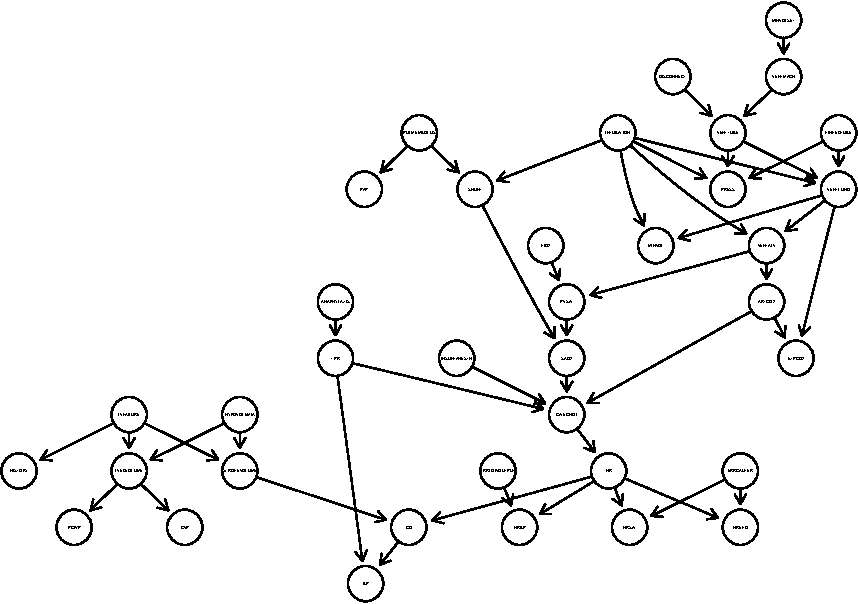
\includegraphics{simulation_bn_files/figure-latex/unnamed-chunk-2-1.pdf}

\hypertarget{convergence}{%
\section{Convergence}\label{convergence}}

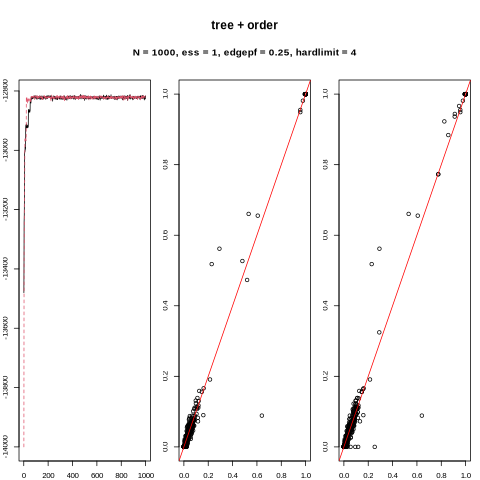
\includegraphics{edgeps_child_tree_order.png}
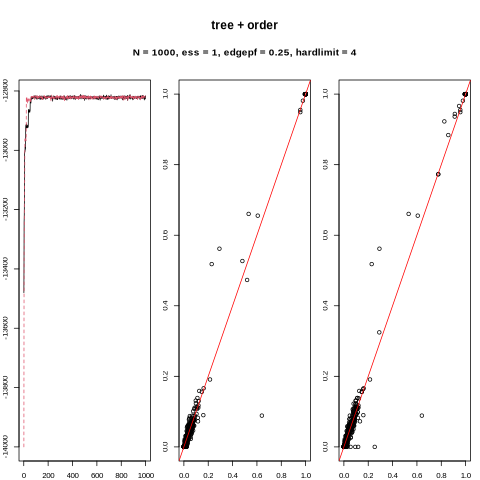
\includegraphics{edgeps_child_tree_order.png}

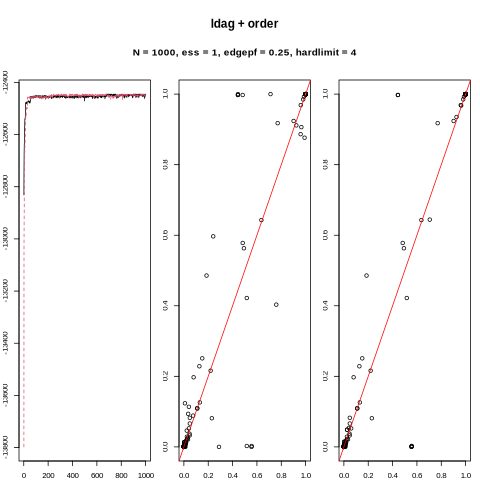
\includegraphics{edgeps_child_ldag_order.png}
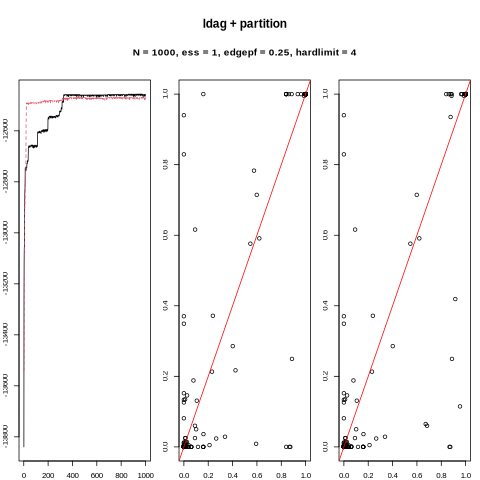
\includegraphics{edgeps_child_ldag_partition.png}

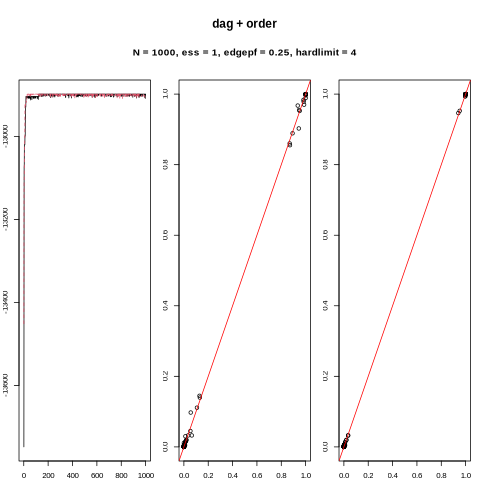
\includegraphics{edgeps_child_dag_order.png =x250}
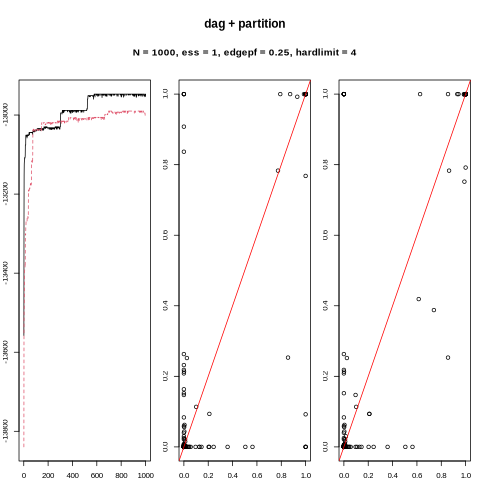
\includegraphics{edgeps_child_dag_partition.png}

\hypertarget{evaluate}{%
\section{Evaluate}\label{evaluate}}

\begin{Shaded}
\begin{Highlighting}[]
\CommentTok{\# evaluate {-}{-}{-}{-}}
\NormalTok{eval\_smpl }\OtherTok{\textless{}{-}} \ControlFlowTok{function}\NormalTok{(smpl, burninsamples, dag, dmat) \{}
\NormalTok{  dindx }\OtherTok{\textless{}{-}} \FunctionTok{diag}\NormalTok{(}\FunctionTok{ncol}\NormalTok{(dag)) }\SpecialCharTok{==} \DecValTok{1} 
  
  \CommentTok{\# list unique DAGs}
\NormalTok{  dags }\OtherTok{\textless{}{-}} \FunctionTok{lapply}\NormalTok{(smpl}\SpecialCharTok{$}\NormalTok{traceadd}\SpecialCharTok{$}\NormalTok{incidence[}\SpecialCharTok{{-}}\NormalTok{burninsamples], as.matrix)}
\NormalTok{  u    }\OtherTok{\textless{}{-}} \FunctionTok{unique}\NormalTok{(dags)}
\NormalTok{  support  }\OtherTok{\textless{}{-}}\NormalTok{ bida}\SpecialCharTok{:::}\FunctionTok{rowsum\_fast}\NormalTok{(}\FunctionTok{rep}\NormalTok{(}\DecValTok{1}\SpecialCharTok{/}\FunctionTok{length}\NormalTok{(dags), }\FunctionTok{length}\NormalTok{(dags)), dags, u)}
\NormalTok{  dags }\OtherTok{\textless{}{-}}\NormalTok{ u }
\NormalTok{  dmats }\OtherTok{\textless{}{-}} \FunctionTok{lapply}\NormalTok{(dags, bida}\SpecialCharTok{:::}\NormalTok{descendants)}
  
\NormalTok{  edgep }\OtherTok{\textless{}{-}} \FunctionTok{Reduce}\NormalTok{(}\StringTok{"+"}\NormalTok{, }\FunctionTok{Map}\NormalTok{(}\StringTok{"*"}\NormalTok{, dags, support))[}\SpecialCharTok{!}\NormalTok{dindx]}
\NormalTok{  ancp  }\OtherTok{\textless{}{-}}  \FunctionTok{Reduce}\NormalTok{(}\StringTok{"+"}\NormalTok{, }\FunctionTok{Map}\NormalTok{(}\StringTok{"*"}\NormalTok{, dmats, support))[}\SpecialCharTok{!}\NormalTok{dindx]}
  
  \CommentTok{\# compute edge prob and ARP}
  \FunctionTok{list}\NormalTok{(}\AttributeTok{edgep =} \FunctionTok{compute\_prec\_recall}\NormalTok{(edgep, dag[}\SpecialCharTok{!}\NormalTok{dindx]),}
       \AttributeTok{ancp =}  \FunctionTok{compute\_prec\_recall}\NormalTok{(ancp, dmat[}\SpecialCharTok{!}\NormalTok{dindx]),}
       \AttributeTok{avgppv =} \FunctionTok{c}\NormalTok{(}\AttributeTok{edgep =} \FunctionTok{avgppv}\NormalTok{(edgep, }\FunctionTok{which}\NormalTok{(dag[}\SpecialCharTok{!}\NormalTok{dindx]}\SpecialCharTok{==}\DecValTok{1}\NormalTok{)),}
                  \AttributeTok{ancp =} \FunctionTok{avgppv}\NormalTok{(ancp, }\FunctionTok{which}\NormalTok{(dmat[}\SpecialCharTok{!}\NormalTok{dindx]}\SpecialCharTok{==}\DecValTok{1}\NormalTok{))))}
\NormalTok{\}}

\NormalTok{compute\_prec\_recall }\OtherTok{\textless{}{-}} \ControlFlowTok{function}\NormalTok{(x, y) \{}
\NormalTok{  indx }\OtherTok{\textless{}{-}} \FunctionTok{order}\NormalTok{(x }\SpecialCharTok{+} \FunctionTok{runif}\NormalTok{(}\FunctionTok{length}\NormalTok{(x))}\SpecialCharTok{/}\DecValTok{1000}\NormalTok{, }\AttributeTok{decreasing =} \ConstantTok{TRUE}\NormalTok{)}
\NormalTok{  tp  }\OtherTok{\textless{}{-}} \FunctionTok{cumsum}\NormalTok{(y[indx])}
  \FunctionTok{cbind}\NormalTok{(}\AttributeTok{x =}\NormalTok{ x[indx], }\AttributeTok{TPR =}\NormalTok{ tp}\SpecialCharTok{/}\FunctionTok{sum}\NormalTok{(y), }\AttributeTok{PPV =}\NormalTok{ tp}\SpecialCharTok{/}\FunctionTok{seq\_along}\NormalTok{(y))}
\NormalTok{\}}

\CommentTok{\# avg ppv }
\NormalTok{avgppv }\OtherTok{\textless{}{-}} \ControlFlowTok{function}\NormalTok{(x, which\_true) \{}
\NormalTok{  np  }\OtherTok{\textless{}{-}}\NormalTok{ (}\FunctionTok{length}\NormalTok{(x)}\SpecialCharTok{{-}}\FunctionTok{rank}\NormalTok{(x}\SpecialCharTok{+}\FunctionTok{runif}\NormalTok{(}\FunctionTok{length}\NormalTok{(x))}\SpecialCharTok{/}\DecValTok{1000}\NormalTok{) }\SpecialCharTok{+}\DecValTok{1}\NormalTok{)  }\CommentTok{\# number of instances with equal to or lower values of x}
\NormalTok{  pp  }\OtherTok{\textless{}{-}}\NormalTok{ np[which\_true]                               }\CommentTok{\# number of positive predictions at each true positive    }
\NormalTok{  ppv }\OtherTok{\textless{}{-}} \FunctionTok{seq\_along}\NormalTok{(pp)}\SpecialCharTok{/}\FunctionTok{sort}\NormalTok{(pp)                       }\CommentTok{\# precision at each positive}
  \FunctionTok{mean}\NormalTok{(ppv)}
\NormalTok{\}}
\end{Highlighting}
\end{Shaded}


\end{document}
